\documentclass[12pt]{article}
\usepackage[utf8]{inputenc}
\usepackage{graphicx}
\usepackage{amsmath}
\usepackage{xcolor}
\usepackage{listings}
\usepackage[margin=1in]{geometry}
\usepackage{hyperref}
\usepackage{caption}
\usepackage{subcaption}
\usepackage{titlesec}
\usepackage{booktabs}
\usepackage{float}
\usepackage{afterpage}

\definecolor{codebg}{rgb}{0.95,0.95,0.95}
\definecolor{myblue}{rgb}{0,0.3,0.6}

\lstset{
    backgroundcolor=\color{codebg},
    basicstyle=\ttfamily\small,
    breaklines=true,
    frame=single,
    numbers=left,
    numberstyle=\tiny\color{gray},
    keywordstyle=\color{myblue},
    commentstyle=\color{green!50!black},
    stringstyle=\color{red},
    showstringspaces=false,
    tabsize=4
}

\title{Car Counting Using Morphological Operations}
\date{\today}

\begin{document}

\maketitle

\begin{abstract}
This document demonstrates a car counting system using morphological image processing techniques. The pipeline includes image preprocessing, binarization, dilation, and connected component analysis to count vehicles in a traffic scene.
\end{abstract}

\section{Libraries Used}
\begin{itemize}
    \item \texttt{numpy}: For numerical operations and array manipulation
    \item \texttt{cv2} (OpenCV): For image processing and computer vision operations
    \item \texttt{matplotlib.pyplot}: For image visualization and plotting
\end{itemize}

\section{Step-by-Step Process}

\subsection{Step 1: Import Libraries}
\begin{lstlisting}[language=Python]
import numpy as np
import cv2 as cv
import matplotlib.pyplot as plt
\end{lstlisting}

\subsection{Step 2: Download Image}
Download the sample traffic image:
\begin{lstlisting}[language=Python]
!wget https://raw.githubusercontent.com/AsadiAhmad/Car-Counter-Morphology/main/Pictures/Cars.jpg -O Cars.jpg
\end{lstlisting}

\subsection{Step 3: Load and Display Image}
Load the image in grayscale and display:
\begin{lstlisting}[language=Python]
cars = cv.imread("Cars.jpg", cv.IMREAD_GRAYSCALE)
plt.imshow(cars, cmap="gray")
\end{lstlisting}

\begin{figure}[H]
    \centering
    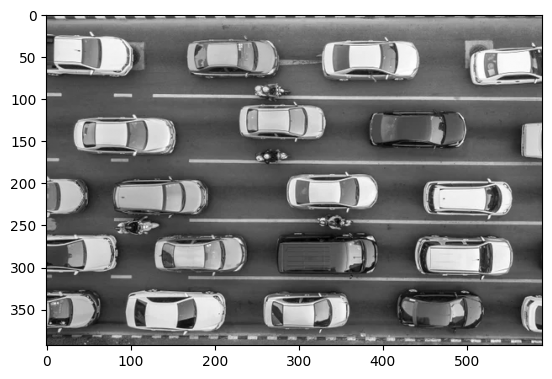
\includegraphics[width=0.8\textwidth]{original_cars.png}
    \caption{Original traffic image}
    \label{fig:original}
\end{figure}

\subsection{Step 4: Crop Image}
Remove unnecessary borders from the image:
\begin{lstlisting}[language=Python]
height, width = cars.shape
cropped_cars = cars[15:height-15, :]
plt.imshow(cropped_cars, cmap="gray")
\end{lstlisting}

\begin{figure}[H]
    \centering
    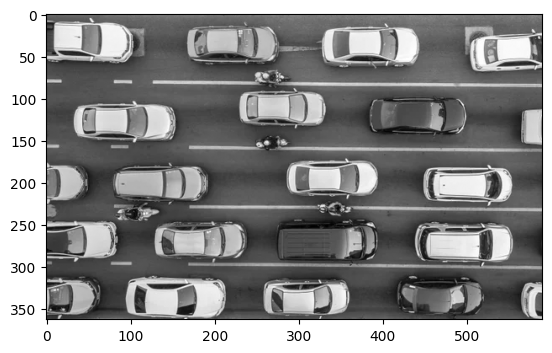
\includegraphics[width=0.8\textwidth]{cropped_cars.png}
    \caption{Cropped image removing top/bottom borders}
    \label{fig:cropped}
\end{figure}

\subsection{Step 5: Blur Image}
Apply Gaussian blur to reduce noise:
\begin{lstlisting}[language=Python]
blurred_cars = cv.GaussianBlur(cropped_cars, (51, 51), 0)
plt.imshow(blurred_cars, cmap="gray")
\end{lstlisting}

\begin{figure}[H]
    \centering
    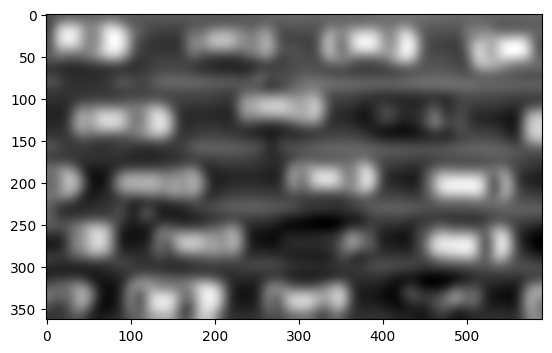
\includegraphics[width=0.8\textwidth]{blurred_cars.png}
    \caption{Image after Gaussian blur (51×51 kernel)}
    \label{fig:blurred}
\end{figure}

\subsection{Step 6: Binarization}
Convert to binary image for morphological processing:
\begin{lstlisting}[language=Python]
bin_cars = np.where(blurred_cars > 127, 255, 0)
plt.imshow(bin_cars, cmap="gray")
scaled_cars = bin_cars.astype(np.uint8)
\end{lstlisting}

\begin{figure}[H]
    \centering
    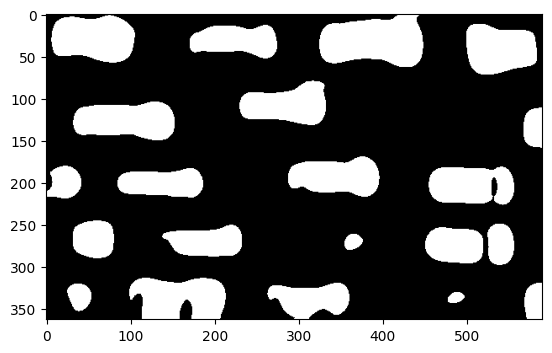
\includegraphics[width=0.8\textwidth]{binary_cars.png}
    \caption{Binarized image (threshold = 127)}
    \label{fig:binary}
\end{figure}

\subsection{Step 7: Dilation for Connecting Car Parts}
Connect car components using dilation:
\begin{lstlisting}[language=Python]
kernel = np.ones((3, 3), np.uint8)
car_dilate = cv.dilate(scaled_cars, kernel, iterations=6)
plt.imshow(car_dilate, cmap="gray")
\end{lstlisting}

\begin{figure}[H]
    \centering
    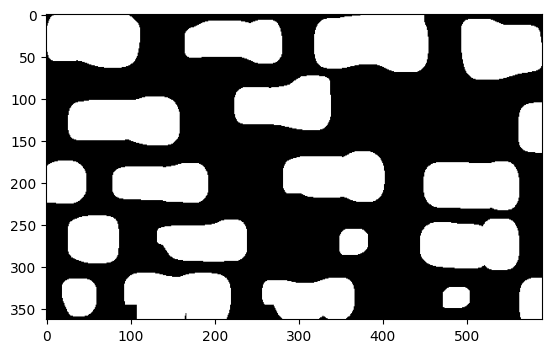
\includegraphics[width=0.8\textwidth]{dilated_cars.png}
    \caption{Image after dilation (6 iterations)}
    \label{fig:dilated}
\end{figure}

\subsection{Step 8: Counting Cars}
Count connected components:
\begin{lstlisting}[language=Python]
num_labels, labels = cv.connectedComponents(car_dilate)
car_count = num_labels - 1  # Subtract background
print(car_count)
\end{lstlisting}

Output:
\begin{verbatim}
20
\end{verbatim}

\subsection{Step 9: Calculating Accuracy}
Calculate counting accuracy:
\begin{lstlisting}[language=Python]
percent = (car_count/21)*100
print(f'{percent:.2f}%')
\end{lstlisting}

Output:
\begin{verbatim}
95.24%
\end{verbatim}

\section{Technical Explanations}

\subsection{Morphological Processing}
\begin{itemize}
    \item \textbf{Cropping}: Removes irrelevant image regions
    \item \textbf{Gaussian Blur}: Reduces noise while preserving edges
    \item \textbf{Binarization}: Simplifies image for morphological operations
    \item \textbf{Dilation}: Connects nearby car parts into single components
    \item \textbf{Connected Components}: Identifies and counts individual cars
\end{itemize}

\subsection{Performance Notes}
\begin{itemize}
    \item 95.24\% accuracy achieved on sample image
    \item Kernel size and iterations affect counting results
    \item Works best with clear separation between vehicles
\end{itemize}

\begin{center}
    \href{https://github.com/AsadiAhmad/Car-Counter-Morphology}{
        \includegraphics[width=0.2\textwidth]{github_logo.png} \\
        \texttt{https://github.com/AsadiAhmad/Car-Counter-Morphology}
    }
\end{center}

\end{document}